%!TEX root = ../thesis.tex
\chapter{Methods}
\label{ch:methods}

\section{Stereo Calibration of the Event Camera and RGB Camera Rig}
\label{sec:stereo-calibration}

The camera rig and recordings analyzed in this thesis originate from the
RGB--DVS stereo camera trap system introduced by
\textcite{gebauer_towards_2024}, who combined an event-based camera
(\textit{DVS}) with a conventional frame-based \textit{RGB} camera observing the same
scene from two viewpoints for real-time insect monitoring in cluttered
outdoor wildlife conditions. Before the two views can be related to one
another, the geometric relationship between the sensors -- their individual
intrinsic parameters and their relative pose -- has to be recovered through
stereo calibration. This section describes that calibration procedure and
motivates every design choice that is not immediate from the standard
calibration literature.

Following their setup, the rig pairs a
Prophesee EVK3 HD event camera (DVS), fitted with a Kowa LM5NCL 4.5\,mm
lens, with a Basler acA1920-150uc RGB camera, fitted with a Kowa LM6JC
6\,mm lens. Per the manufacturers' datasheets, the two sensors have a pixel
pitch of $4.86\,\mu\text{m}$ (DVS) \parencite{prophesee_evk3hd_2024} and
$4.8\,\mu\text{m}$ (RGB) \parencite{basler_aca1920_2026}, at native
resolutions of $1280\times720$ (DVS) and $1920\times1200$ (RGB).
Consequently, the two sensors also differ in aspect ratio. The physical
baseline between the two camera housings was measured directly as
$60\,\text{mm}$ \parencite{gebauer_towards_2024}; this value is used in Section~\ref{sec:scale-recovery} to
resolve the scale ambiguity inherent to the calibration.

At a high level, calibration proceeds as follows: (1) detect a planar
calibration target in both video streams, (2) pair up detections that occur
at corresponding frames, (3) calibrate each camera individually, (4)
calibrate the pair jointly while keeping the individual intrinsics fixed,
(5) discard the frame pairs with the worst geometric consistency and refit,
and (6) rectify both views onto a common image plane. Each step is discussed
below.

\subsection{Calibration Target and Detection}

A planar \textit{asymmetric circle grid} (4 columns $\times$ 11 rows,
staggered; see Figure~\ref{fig:stereo-calib-board}) was used as the calibration target, detected via blob-based grid
detection rather than the more common checkerboard corner detection.

\begin{figure}[ht]
    \centering
    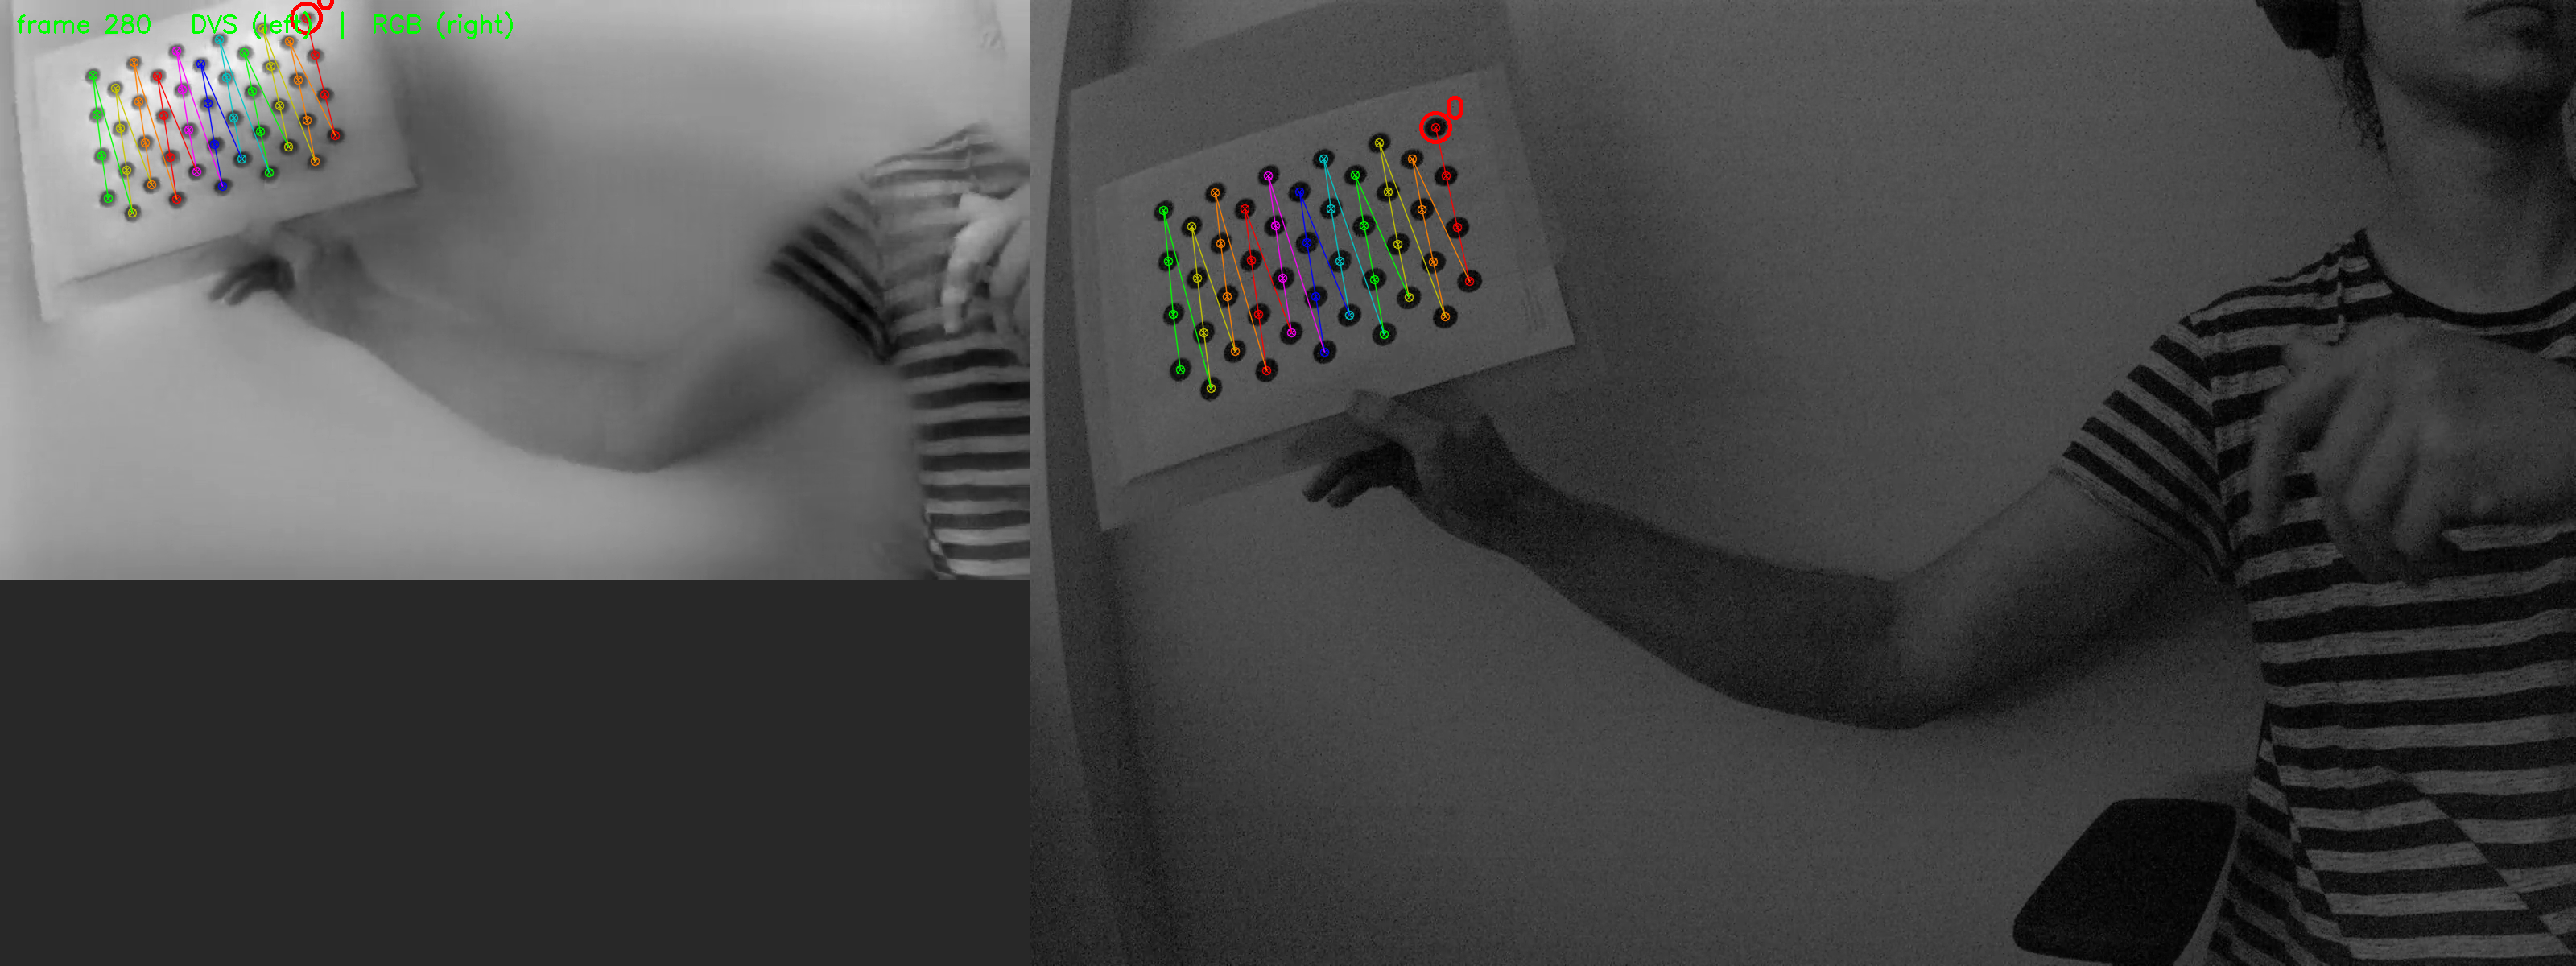
\includegraphics[width=\textwidth, height=\textheight, keepaspectratio]{figures/verify_02_frame280.png}
    \caption{Detected asymmetric circle grid in a synchronized DVS (left)
    and RGB (right) frame pair (frame 280), color-coded per row by
    \texttt{cv2.findCirclesGrid}; the origin point is circled in red.}
    \label{fig:stereo-calib-board}
\end{figure}

Compared to a checkerboard, an asymmetric circle grid removes the
$180^\circ$ pose ambiguity that a fully symmetric pattern is subject to,
without requiring an additional fiducial marker
\parencite{opencv_calibration_pattern_docs}. Circle centroids are also
comparatively robust to defocus \parencite{choi_robust_2021}, which is
relevant here because the DVS "frames" fed into the detector are not raw
camera frames. They are reconstructed from the asynchronous event stream
and are consequently noisier and lower-contrast than a conventional
photograph \parencite{gallego_event-based_2022}. The blob-detector
thresholds (minimum area, circularity, convexity, and inertia ratio) were
loosened relative to their defaults for the same reason, so that
imperfectly round blob edges from the reconstructed DVS frames are still
accepted, while area filtering still rejects spurious detections.

\subsection{Temporal Synchronization}
\label{sec:sync}

Detections from the two videos are paired purely by integer frame index:
frame $N$ of the DVS recording is assumed to correspond to frame $N$ of the
RGB recording. This is only valid if the two recordings are already
frame-rate-matched and phase-aligned before calibration -- guaranteed here
by hardware-triggered, pre-synchronized capture -- rather than something the
calibration procedure itself establishes. Converting the event stream into a
conventional frame sequence and feeding it into unmodified, standard
frame-based calibration tooling, rather than calibrating directly on raw
events, follows the approach of \textcite{muglikar_how_2021}, who use the same
strategy and explicitly rely on a hardware-synchronized trigger between the
event sensor and the reference camera for their frame-index-based pairing.

\subsection{Camera Model and Initial Intrinsics}

Both cameras are modeled as pinhole cameras with radial and tangential lens
distortion. Rather than letting the calibration solver estimate the initial
intrinsic parameters purely from the observed correspondences, the initial
camera matrix for each sensor is constructed directly from its known optics:
given a focal length $f$ (mm) and pixel pitch $p$ (\textmu m), the initial
focal length in pixels is
\begin{equation}
    f_\text{px} = \frac{f \cdot 1000}{p},
\end{equation}
with the principal point initialized to the image center. Seeding the
optimizer with a physically plausible starting point rather than starting
from scratch matters most when only a small number of calibration views is
available, since an unconstrained solve is more likely to diverge under
those conditions -- the same reasoning that motivates the closed-form
initial estimate preceding nonlinear refinement in \textcite{zhang2000}'s
own calibration method.

\subsection{Two-Stage Calibration: Individual, Then Joint}

Each camera is first calibrated individually from its own detected
correspondences, and only afterwards is a joint stereo calibration performed
with both cameras' intrinsics held fixed, solving only for the relative
rotation $R$ and translation $T$ between them. This two-stage order --
individual intrinsic calibration before joint extrinsic calibration -- is
the standard recommended practice, since solving for intrinsics and
extrinsics simultaneously is a substantially higher-dimensional problem that
is more prone to diverging under noisy correspondences
\parencite{opencv_calib3d_docs}. Both the individual and the joint
calibration are instances of \textcite{zhang2000}'s planar calibration
method, which is precisely why a planar target is sufficient here rather
than a three-dimensional calibration rig.

An optional 8-parameter rational distortion model (in place of the default
5-parameter polynomial model), following \textcite{claus_rational_2005}, is
available for lenses whose distortion the basic model cannot capture well,
at the cost of requiring more calibration views to fit the additional free
parameters reliably; it was treated as an opt-in rather than the default for
that reason.

\subsection{Outlier Rejection via Symmetric Epipolar Error}
\label{sec:outlier-rejection}

The frame pairs surviving the initial joint calibration are scored by their
\emph{symmetric epipolar error}: for each pair's correspondences, points
are projected into the fundamental matrix's epipolar lines in the
respective other image, and the mean point-to-line distance is averaged
over both directions (Section~\ref{sec:epipolar-geometry} introduces the
epipolar line and the fundamental matrix $F$ that produces it, in full).
Because both cameras are already individually and jointly calibrated at
this point in the pipeline, $F$ falls out directly from that calibrated
solve, $F = K'^{-\top}[T]_\times R\,K^{-1}$, rather than requiring separate
estimation from raw point correspondences the way
Section~\ref{sec:epipolar-geometry} describes in general. This is a true
geometric (pixel) distance rather than an
algebraic residual, which is precisely why it is a standard criterion for
judging the quality of an estimated fundamental matrix
\parencite{fathy2011}. The worst-scoring 20\,\% of frame pairs are then
discarded and the stereo calibration is refit on the remaining pairs. This
exclusion criterion is available immediately after the first stereo solve,
rather than requiring a second full bundle-adjustment pass to obtain a
per-image reprojection error. A minimum of 10 synchronized frame
pairs was treated as the threshold below which the calibration is flagged as
potentially unreliable.

\subsection{Stereo Rectification}
\label{sec:stereo-rectification}

Given the final calibrated intrinsics, distortion coefficients, and relative
pose, both views are rectified onto a common image plane: a rotation is
applied to each camera such that the two image planes become coplanar and
row-aligned, so that corresponding points in the two rectified images share
the same row coordinate. \textcite{fusiello2000} give a compact, direct
linear method for computing such rectifying transformations from the two
camera projection matrices, without requiring iterative optimization, and
show that the resulting loss of accuracy in subsequent 3D reconstruction is
negligible compared to more elaborate rectification schemes; this is the
approach used here. The valid-pixel region is cropped rather than padded
with black borders, trading field of view for the guarantee that every
pixel in the rectified output has valid source data.

\subsection{Metric Scale Recovery}
\label{sec:scale-recovery}

The physical spacing between adjacent circles on the calibration target was
not measured in absolute units; the target's object points were instead
defined in arbitrary grid-step units. Camera calibration recovers geometry
only up to the units in which the object points are given
\parencite{zhang2000}, so the estimated translation $T$ between the two
cameras is likewise recovered only up to an unknown scale factor, not
directly in millimeters. Because the physical baseline between the two
camera housings is known independently (measured as $60\,\text{mm}$,
Section~\ref{sec:stereo-calibration}), that single external measurement is
used to resolve the ambiguity after the fact:
\begin{equation}
    \text{scale} = \frac{60\,\text{mm}}{\lVert T \rVert}.
\end{equation}
This is the same scale ambiguity already noted for the essential matrix in
Section~\ref{sec:essential-fundamental-matrices} \parencite{longuet-higgins_computer_1981}
-- whenever a vision system's reconstruction is correct only up to scale, a
single known real-world length is used to fix it after the fact, most
notably in monocular structure-from-motion. It avoids having to measure the
sub-millimeter dot spacing on the physical target directly, at the cost of
the recovered scale depending on how accurately the $60\,\text{mm}$ baseline
itself was measured.

\section{Constructing a Probability Zone Around the Epipolar Line}
\label{sec:probability-zones}

The calibration and rectification pipeline described above resolves the
correspondence problem between the two views down to a single degree of
freedom: for a DVS detection at rectified row $v_0$, the corresponding RGB
point is guaranteed, by construction of rectification, to lie on the same
row, regardless of the insect's unknown depth. What rectification does
\emph{not} resolve is exactly where on that row the correspondence falls --
that position is fixed by the insect's depth, which is not known -- nor does
it guarantee that the true row is exactly $v_0$, since $v_0$ is itself only
as accurate as the calibration and rectification it depends on. The current
implementation (Section~\ref{sec:outlier-rejection}) treats $v_0$ as exact
and leaves the position along the row completely unconstrained; it draws a
single-pixel line for visual verification, not a region a detector could
search. This section formalizes the two remaining sources of uncertainty
separately -- a small one \emph{across} the row and a much larger one
\emph{along} it -- and combines them into a single two-dimensional
probability zone, rather than a one-dimensional distribution confined to the
line itself, since there is no guarantee the true correspondence sits
exactly on the line either.

\subsection{Across-Line Uncertainty}
\label{sec:zone-across-line}

Deviation of the true corresponding row $v$ from the assumed row $v_0$ is
modeled as zero-mean Gaussian,
\begin{equation}
    p_\perp(v) = \mathcal{N}\left(v;\, v_0,\, \sigma_\perp^2\right),
\end{equation}
reflecting residual calibration and rectification error rather than any
property of the scene. \textcite{zhang_determining_1998} derives this kind
of uncertainty formally, by propagating correspondence noise through the
estimated fundamental matrix to first order, and shows that it is not
spatially uniform: it grows large near the epipole and depends on the local
distribution of correspondences used to estimate $F$. A practical estimate
of $\sigma_\perp$ is already available without any new measurement: the mean
symmetric epipolar error computed for outlier rejection in
Section~\ref{sec:outlier-rejection} \parencite{fathy2011} is exactly this
residual, averaged over the calibration frame pairs. Using it as a single,
constant $\sigma_\perp$ for the whole image is an approximation -- per
\textcite{zhang_determining_1998}, the true uncertainty varies with position
-- but a reasonable one within the comparatively narrow field of view and
fixed working distance of a stationary camera trap, and considerably better
motivated than an arbitrarily chosen band width.

\subsection{Along-Line Uncertainty}
\label{sec:zone-along-line}

The column $u$ at which the correspondence falls on row $v_0$ is fixed by
disparity $d = u - u_{\text{DVS}}$, which relates to depth $Z$ for a
rectified pair with focal length $f$ and baseline $B$
(Section~\ref{sec:scale-recovery}) by the standard relation
$d = fB/Z$ \parencite{hartley_multiple_2003}. Two distinct cases have to be
distinguished here, since they justify different distributions for
$p_\parallel(u)$:

\begin{itemize}
    \item \textbf{No prior track.} On a first detection, nothing
    distinguishes one depth within the trap's working range
    $[Z_{\min}, Z_{\max}]$ from another, so there is no principled center
    for a Gaussian. The corresponding disparity range
    $[d_{\min}, d_{\max}] = [fB/Z_{\max}, fB/Z_{\min}]$ instead bounds a
    uniform distribution over $u$. \textcite{kendall_end-to-end_2017}
    avoid assuming a shape for this distribution altogether: their GC-Net
    builds a cost volume over all candidate disparities and takes a
    differentiable soft-argmin over it, learning the along-line
    distribution from data rather than presupposing it is Gaussian or
    uniform.
    \item \textbf{Established track.} Once a track exists, a motion model
    predicts a specific disparity and its own uncertainty, and a Gaussian
    centered on that prediction is well justified. Folding a predicted
    position and its uncertainty into a bounded search region for the next
    measurement -- rather than hard-gating to whichever detection happens
    to fall nearest the prediction -- is exactly the problem addressed by
    joint probabilistic data association \parencite{fortmann_sonar_1983},
    which weights every measurement inside the gate by its probability
    instead of committing to the single closest one.
\end{itemize}

\subsection{Interfacing the Zone with YOLO}
\label{sec:zone-yolo-interface}

Combining both components under an independence assumption gives a single
zone density, $p(u, v) = p_\parallel(u) \cdot p_\perp(v)$, but this alone
does not specify how the zone should act on YOLO. At least three
architecturally different options exist, and the choice among them is not
yet settled:

\begin{enumerate}
    \item \textbf{Input-level masking or cropping.} The RGB frame is
    darkened or cropped outside the zone before detection. Cheap, but a
    misestimated zone permanently removes evidence YOLO could otherwise
    have used.
    \item \textbf{Post-hoc re-weighting.} YOLO runs unmodified, and its
    output detections are re-ranked by the zone density evaluated at their
    location. Non-invasive, but presupposes YOLO's objectness-times-class
    score is a calibrated probability, which it is not by default --
    \textcite{hall_probabilistic_2020} address exactly this by representing
    a detector's own spatial uncertainty as Gaussian-distributed box
    corners (PBox) rather than fixed points, evaluated with their PDQ
    metric instead of plain IoU.
    \item \textbf{Soft-label training.} The zone is folded into the loss
    directly, so the network learns calibrated positional confidence
    itself. \textcite{choi_gaussian_2019} take this approach for YOLOv3,
    predicting a Gaussian (mean and variance) per box coordinate and
    training it with a negative log-likelihood loss, which reduced false
    positives without a separate re-weighting step; \textcite{law_cornernet_2020}
    similarly reduce the training penalty smoothly around keypoints with a
    Gaussian rather than a hard positive/negative split. More invasively,
    \textcite{he_epipolar_2020} and \textcite{liu_when_2023} build the
    epipolar constraint directly into a network's attention, letting each
    location attend only to a soft neighborhood along the corresponding
    epipolar line in the other view instead of the whole image -- the
    same restriction this section proposes, but learned end-to-end rather
    than computed from calibration statistics. A less invasive stereo
    precedent specifically for detection, rather than pose or multi-view
    stereo, is \textcite{li_stereo_2019}'s Stereo R-CNN, which keeps left
    and right region proposals separate rather than fusing them into a
    single soft zone, and instead reconciles them afterwards by
    photometric alignment -- a reminder that a hard, symbolic stereo
    constraint remains a competitive alternative to a soft probabilistic
    one even in recent detection literature.
\end{enumerate}

\todo{Decide which of the three interfacing options above this thesis
implements, and update this section accordingly once that decision is
made.}

\subsection{Known Limitations}
\label{sec:zone-limitations}

Three issues remain open regardless of which interfacing option is chosen.
First, if the zone is used to generate soft training labels, weighting
crops by a Gaussian centered on the annotated ground truth risks teaching
the network to exploit the label's position rather than the insect's
appearance -- the geometric prior needs to stay auxiliary to appearance-based
evidence, not a substitute for it. Second, if the along-line Gaussian is
ever centered on a track's own previous prediction with no independent
check, errors can compound and the track can lock onto clutter; this is the
classical failure mode nearest-neighbor gating has, and the reason
\textcite{fortmann_sonar_1983}'s joint probabilistic data association
weights all measurements in the gate instead of committing to one. Third,
the zone is asymmetric by construction: the DVS view triggers the candidate
row through motion, while the zone itself and any resulting detection are
constructed entirely in the rectified RGB view -- a distinction worth
keeping explicit, since "the epipolar line" otherwise reads as a single,
sensor-agnostic object when it is not.
